% ================================== HEADER ====================================
\documentclass{article}           % Sets style/look of many things.
% \documentclass{report}          % part, chapters, front page etc.
\usepackage{exsheets}
\usepackage[utf8]{inputenc}       % Encoding of input files UTF-8
\usepackage[T1]{fontenc}
\usepackage[scaled]{beramono}     % Font
\usepackage{color}                % Color text
\usepackage{titlesec}             % Select alternative section titles
\usepackage{fancyvrb}
\usepackage{verbatim}             % Comment environment
\usepackage{listings}             % Format and render text/code etc.
\usepackage{minted}               % Much better syntax highlighting
\usepackage{float}                % Control of floating environment/figure
\usepackage{graphicx,  subfigure} % Better figures, graphics, units etc.
\usepackage{multicol}             % Multiple columns
\usepackage{amsmath}              % Math: Equation, split, align etc.
\usepackage{siunitx}              % SI units
\usepackage{mathtools}            % Different math tools to use with amsmath
\usepackage{amssymb}              % Math symbols
\usepackage[
    colorlinks,
    citecolor=black,              % I like links with standard black color
    filecolor=black,
    linkcolor=black,
    urlcolor=black
]{hyperref}                       % Links in TOC etc.
\usepackage[all]{hypcap}          % Better links to floating environment

\usepackage{tabto}
\newcommand\marginsymbol[1][0pt]{%
\tabto*{0cm}\makebox[\dimexpr-1cm-#1\relax][r]{$\mathbb{P}$}\tabto*{\TabPrevPos}}

\renewcommand{\thesubsection}{\thesection.\alph{subsection}}
\title{\vspace{-2cm}INF3490/INF4490 Mandatory Assignment 2:\\
Multilayer Perceptron}
\author{Eivind Samuelsen, Ole Herman S. Elgesem}

\date{\today}

% Removing paragraph indents is sometimes useful:
%\setlength\parindent{0pt}

% Make margins smaller to fit more figures, tables etc on page: (optional)
\addtolength{\oddsidemargin}{-0.8in}
\addtolength{\evensidemargin}{-0.8in}
\addtolength{\textwidth}{1.6in}
\addtolength{\topmargin}{-0.8in}
\addtolength{\textheight}{1.6in}
% ==============================================================================

% ================================= DOCUMENT ===================================
\begin{document}
    \renewcommand\marginsymbol[1][0pt]{%
  \tabto*{0cm}\makebox[-1cm][c]{$\mathbb{P}$}\tabto*{\TabPrevPos}}

\maketitle
\section*{Rules}
This is an individual assignment.
You are not allowed to deliver together or copy/share source-code or answers with others.
Before you begin the exercise, review the rules at this website:
\begin{center}
\url{http://www.uio.no/english/studies/admin/compulsory-activities/mn-ifi-mandatory.html}
\end{center}


The assignment can be changed/updated after release (to clarify or correct mistakes).
It is advised to always use the latest version, available
 \href{http://www.uio.no/studier/emner/matnat/ifi/INF3490/h16/assignment-2/inf3490-as2.pdf}{\textbf{here}}.

\section*{Delivering}
\textbf{Deadline:} 2016-10-31 23:59:00. All deliveries must be made through
\href{https://devilry.ifi.uio.no}{\textbf{Devilry}}.
\section*{What to deliver?}
Deliver one single zipped folder (.zip, .tgz or .tar.gz) which includes:
\begin{itemize}
    \item PDF report containing:
    \begin{itemize}
        \item Your name and username (!)
        \item Instructions on how to run your program.
        \item Answers to all questions from assignment.
        \item \emph{Brief} explanation of what you've done.
    \end{itemize}
    \item Source code
    \item Data file (so the program can run \emph{right away})
    \item Any files needed for the group teacher to easily run your program on
          IFI linux machines.
\end{itemize}
\emph{Important: } if you weren't able to finish the assignment, use the PDF
report to elaborate on what you've tried and what problems you encountered.
Students who have made an effort and attempted all parts of the assignment
will get a second chance even if they fail initially. This exercise will be
graded PASS/FAIL.

\subsection*{Preface}
The purpose of this assignment is to give you some experience applying supervised learning with a multilayer perceptron (MLP).
In order to control a robotic prosthetic hand, Prosthetic hand controllers (PHCs) reads the electromyographic signals generated by contracting muscles in the under arm.
The idea is that we can, through supervised learning, get a PHC to learn which hand movement the user of a robotic prosthetic hand wants to perform.

\begin{center}
    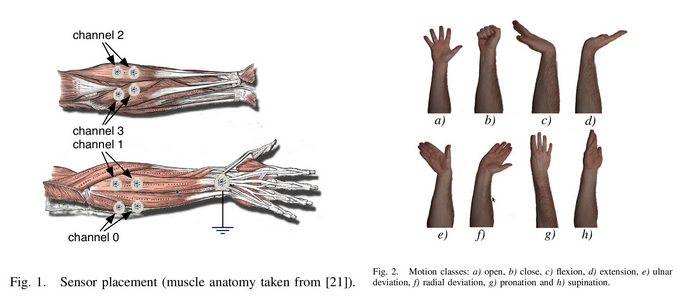
\includegraphics[scale=0.8]{figures/handfigures.png}
\end{center}

\subsection*{The data}
 The data you will be classifying
are electromyographic (EMG) signals corresponding to various hand
motions, collected over three days (one dataset per day).\footnote{
See section 2 of K. Glette, J. Torresen, Thiemo Gruber, Bernhard Sick,
Paul Kaufmann, and Marco Platzner. \emph{Comparing Evolvable Hardware
to Conventional Classifiers for Electromyographic Prosthetic Hand
Control}. (In Proceedings of the 2008 NASA /ESA Conference on Adaptive
Hardware and Systems(AHS-2008), Noordwijk, The Netherlands, IEEE Computer
Society, 2008, or \url{http://folk.uio.no/kyrrehg/pf/papers/glette-ahs08.pdf})
if you are curious about how the data was collected.
} Each row of the data has 40 features (4 sensors, 10 readings each) and one classification value (1-8, corresponding to
the 8 hand motions.\footnote{
Which, for the curious, are: open, close, flexion, extension, ulnar
deviation, radial deviation, pronation, and supination
}). You can get the \href{http://www.uio.no/studier/emner/matnat/ifi/INF3490/h16/assignment-2}{\textbf{data}}(.zip or .tgz) from the \href{http://www.uio.no/studier/emner/matnat/ifi/INF3490/h16/index.html}{\textbf{semester page}}.


\subsection*{Getting started}

You are free to use a programming language of your own choice, but we strongly recommend using Python.
The precode is only available in Python (the files \emph{movements.py} and \emph{mlp.py} that are bundled with the data).
If you choose another language, you will have to implement everything yourself.
Along with the two precode files, you are also given four files with data:
\begin{itemize}
\item \emph{data/movements\_day1.dat}
\item \emph{data/movements\_day2.dat}
\item \emph{data/movements\_day3.dat}
\item \emph{data/movements\_day1-3.dat}
\end{itemize}
As the last file contains data for all days, you don't \emph{have to} use the other files.
You can use the \emph{movements\_day1-3.dat} file and split up the data into different sets.\\


The file \emph{movements.py} will read one specified data file, and split it into training, validation and test sets. Then it will create an MLP, run the training on the MLP and call the confusion method of the MLP to print the confusion matrix.

\noindent A class mlp with four methods is given in the file \emph{mlp.py}:

\begin{itemize}
\item \emph{earlystopping}
\item \emph{train}
\item \emph{forward}
\item \emph{confusion}
\end{itemize}

\noindent \emph{earlystopping} is the method that starts the training of the network and keeps track of when to stop the training. It should, in each iteration, call MLPs train method and run the network forward. Before the network learns the trainingdata too well, we stop training to avoid overfitting. See Fig. 4.11 on page 88, S. Marsland.\\

\noindent \emph{train} trains the network. This means running the backwards phase of the training algorithm to adjust the weights. See section 4.2.1 on page 77-79, S. Marsland.\\

\noindent \emph{forward} run the network forward. When running the network forward, a perfect classifier should always have the highest value on the correct output. You will experience that this is not the case the first time(s) the network is run forward, which is why you are adjusting the weights in train.\\

\noindent \emph{confusion} prints a confusion matrix. Run the network forward with the test set, and fill out the outputs in a matrix. The matrix should be a $c \times c$ matrix (where $c$ is the number of classes), and have the correct classes on one axis and classified classes on the other axis. Print also the percentage of correct classes.


\begin{figure}
    \centering
    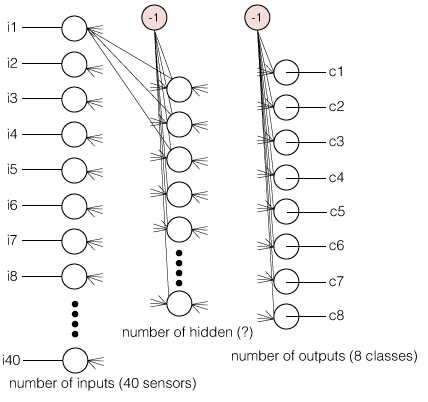
\includegraphics[scale=0.5]{figures/neuralnet.png}
    \caption{The neural net with one hidden layer}
    \label{fig:awesome_image}
\end{figure}

\subsection*{How the algorithm runs}
After the input is given to the MLP, we start to train the network. Instead of running the training a fixed number of iterations, we split it up into parts, where we decide whether to stop in between the iterations. This means that we will first check if the error of the network with a validation set in \emph{earlystopping}, and if our stopping criteria is not met, we start to train the network.

The training phase consists of the first running the network forwards, then running it backwards, adjust the weights and repeat for as many iterations as we have chosen (10,100,1000). When training is done we return to \emph{earlystopping} to check if we're done.

Once we're done we print out the confusion table based on how the network classified the data in the test set.

\begin{figure}[h]
    \centering
    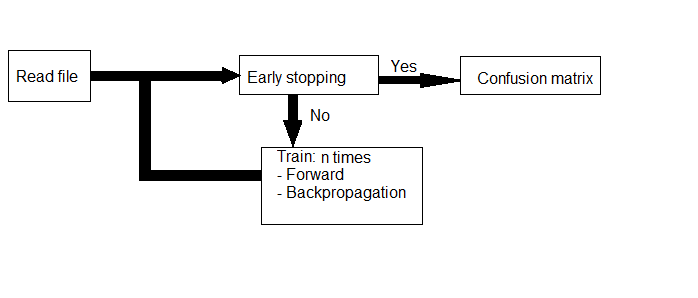
\includegraphics[scale=0.5]{figures/diagram.png}
    \caption{A diagram of how the algorithm runs}
    \label{fig:awesome_image}
\end{figure}

\subsection*{What to do}

\subsubsection*{All students}
\begin{itemize}
\item Implement the neural net as explained above. Don't use more than one hidden layer (see Fig. 1).
\item Run the algorithm on dataset \emph{movements\_day1-3.dat}. You should test with at least three different number of hidden nodes (e.g 6, 8, 12). Report your findings and provide the resulting confusion tables with percentages, one for each net with different number of hidden nodes. How many nodes do you find sufficient for the network to classify well?
\item By only looking at your reported confusion tables, which classes where likely to be mistaken for each other?
\end{itemize}

\subsubsection*{INF4490}
\begin{itemize}
\item Implement k-fold cross-validation. Choose a suitable k. Report the correct percentages for each fold, along with the average and standard deviation. Please do not include all confusion tables in your report.
\end{itemize}

\subsubsection*{Frequently Asked Questions(FAQ)}
\textit{What should my datastructure look like?}

You are free to implement a datastructure of your own choice.
In this mandatory assignment you are implementing a neural net with one hidden layer.
That means you will have two weight layers with floats
(one between input and hidden, and one between hidden and output).
These two weight layers together constitute the neural network and it’s basically the only datastructure you need.
We recommend that you simply use numpy matrices or numpy 2D arrays.
Keep in mind that you need some additional structures to handle inputs, outputs, etc.\\

\noindent
\textit{I think I am done, but my neural net performs poorly (less than 60\% accuracy), why?}

Make sure you’re not using a sigmoid activation function on the output.
If you used Eq. 4.7 from the book, replace it with a linear output (Eq. 4.13).
When replacing this output function, you also need to change the error function accordingly;
use eq. 4.14 instead of eq. 4.8.\\

\noindent
\textit{What is one iteration in training?
Is it one run with one input vector or is it running the whole training set through the net?}

The training data is an array of n input vectors,
and there are multiple ways to feed this through and update the network.
You are free to define an iteration how you want,
but make sure you train on all data.
Here are three possible methods:
\begin{enumerate}

    \item   Feed the network with the whole training set.
            Then update the weights based on the n output errors.
            This is one iteration.

    \item   Feed the network with one input vector from the training set.
            Update the weights.
            Repeat until you’ve been through the training set.
            When done with the whole training set, you have one iteration.
            This method differs from 1. in the way that weights will be updated after every input from the training set.
            Now the order matters because training vector n will be run on a network trained on all the other vectors in the same iteration (and vector 1 will always be first in each iteration).
            In order to avoid this problem, the order of the training data should be randomized before each iteration.

    \item   Pick a random vector from the training set and feed it into the net, update the weights.
            Let’s call this one iteration, but keep in mind that you need n times more iterations in order to get the same amount of training as in 1. and 2.
            This method is similar to 2., but instead of running one iteration over the whole set,
            we randomly pick one by one vector.
            This means that some vectors may never be chosen and some vectors might be used multiple times.

\end{enumerate}

\noindent
\textit{What libraries am I allowed to use?}

You are not allowed to use machine learning libraries,
as you have to \emph{implement} the algorithm yourself as explained in this assignemnt.
General purpose/scientific libraries for calculations, plotting etc. are allowed.

\subsubsection*{Precode}
The assignment folder includes some precode that you're encouraged to use.
Modify \texttt{mlp.py} and run \texttt{movements.py}:
\begin{center}
    \texttt{[olehelg@vetur code]\$ python3 movements.py}
\end{center}

\subsubsection*{movements.py}
\inputminted{Python}{./code/movements.py}

\subsubsection*{mlp.py}
\inputminted{Python}{./code/mlp.py}

\section*{Contact and Github}
Corrections of grammar, language, notation or suggestions for improving this material are appreciated.
E-mail me at \href{mailto:olehelg@uio.no}{\textbf{olehelg@uio.no}} or use \href{https://github.com/olehermanse/INF3490-AI_Machine_Learning}{\textbf{GitHub}} to submit an issue or create a pull request.
The \href{https://github.com/olehermanse/INF3490-AI_Machine_Learning}{\textbf{GitHub repository}} contains all source code for assignments, exercises, solutions, examples etc.
As many people have been involved with writing and updating the course material, they are not all listed as authors here.
For a more complete list of authors and contributors see the \href{https://github.com/olehermanse/INF3490-AI_Machine_Learning/blob/master/README.md}{\textbf{README}}.


\end{document}
% ==============================================================================
